Viele Probleme der KI lassen sich auf eine systematische Suche in einem Wurzelbaum reduzieren. \\
Problem: Riesige Anzahl von Knoten in typischen Suchbäumen. 
\cparagraph{Beispiel} Schachspiel, ca. $30$ Möglichkeiten pro Halbzug (Zug einer Farbe). Bei $50$ Halbzügen enthält der Suchbaum:
$$\sum_{d=0}^{50} 30^d = \frac{30^{51}-1}{30-1} \approx 7,4 \cdot 10^{73}\unit{Knoten}$$
Bei $10\, 000$ Computern, die $10^9 \unit{Knoten/s}$ erzeugen und durchsuchen können, würde das durchsuchen so lange dauern:
$$ \frac{7,4 \cdot 10^{73}}{10\,000 \cdot 10^9}\unit{s}=2,3 \cdot 10^{53} \unit{Jahre}$$

\section{Uninformierte Suche}
Bereits bekannt: Breiten- und Tiefensuche. Zur Implementierung in Prolog benötigen wir:
\begin{itemize}
\item \lstinline`findall(X, P, L)`: Sucht alle \lstinline`X`, für die \lstinline`P` wahr ist und erzeugt daras die Liste \lstinline`L`.
\item \lstinline`not(P)`: Ist wahr genau dann, wenn Prolog \lstinline`P` nicht beweisen kann („Negation by failure“).
\end{itemize}
\subsection{Breitensuche}
\begin{lstlisting}[language=Prolog]
% Adjazenzrelation des ungerichteten Graphen (nicht effizient)
adj(X,Y) :- adj0(X,Y); adj0(Y,X).
adj0(X,Y) :- member((X,Y), [(1,2), (2,4), (2,5), (3,4), (3,6), (4,5)]).

goal(6).

% Breitensuche
bfs([H|T], Discovered) :-
	goal(H);
	findall(Node, (adj(H, Node), not(member(Node, Discovered))), NewNeighbors),
	append(T, NewNeighbors, Queue),
	append(Discovered, NewNeighbors, Dc),
	write('Queue: '), writeln(Queue), % zur Illustration
	bfs(Queue, Dc).
\end{lstlisting}

Starten der Breitensuche beim Knoten $1$:
\begin{lstlisting}[language=Prolog]
?- bfs([1], [1]).
Queue: [2]
Queue: [4,5]
Queue: [5,3]
Queue: [3]
Queue: [6]
true .
\end{lstlisting}
\subsection{Problem der Breiten- und Tiefensuche} 
Wenn alle bereits besuchten Knoten gespeichert werden: Exponentielle Laufzeit und exponentieller Speicherplatzbedarf (für die Discoverd-Liste) in der Tiefe des Baumes.
\subsection{Tiefensuche}
Einfach: aus \lstinline`append(T, NewNeighbors, Queue)` wird \lstinline`append(NewNeighbors, T, Queue`.\\
Ohne expliziten Stack, Knoten auf aktuellen Pfad werden gespeichert (nicht alle Knoten wie bei Discovered $\to$ vermeidet exponentiellen Speicherplatzbedarf -- funktioniert, da der zu durchsuchende Graph in der Regel ein Baum ist [Knoten könnten nur durch Schleifen doppelt besucht werden]):
\begin{lstlisting}[language=Prolog]
% Adjazenzrelation des ungerichteten Graphen (nicht effizient)
adj(X,Y) :- adj0(X,Y); adj0(Y,X).
adj0(X,Y) :- member((X,Y), [(1,2), (2,4), (2,5), (3,4), (3,6), (4,5)]).

goal(6).

dfs3(Node, Path) :-
	goal(Node);
	adj(Node, NewNeighbor), not(member(NewNeighbor,Path)),
	write('Knoten: '), writeln(NewNeighbor), % zur Illustration
	dfs3(NewNeighbor, [NewNeighbor|Path]).

% Wie dfs3, gefundener ReturnPath wird zurückgegeben
dfs4(Node, Path, ReturnPath) :-
	goal(Node), reverse(Path, ReturnPath);
	adj(Node,NewNeighbor), not(member(NewNeighbor,Path)),
	dfs4(NewNeighbor, [NewNeighbor|Path], ReturnPath).
\end{lstlisting}

\subsection{Vorteile/Nachteile Breiten- und Tiefensuche}
\lecdate{22.05.2017}
\subsubsection*{Breitensuche}
\begin{itemize}
\item[$+$] Liefert kürzesten Pfad, funktioniert auch für unendliche Graphen.
\item[$-$] Alle Knoten werden gespeichert.
\end{itemize}

\subsubsection*{Tiefensuche}
\begin{itemize}
\item[$+$] Nur die Knoten auf dem aktuellen Pfad werden gespeichert.
\item[$-$] Liefert nicht immer den kürzesten Pfad und funktioniert nicht für unendliche Graphen.\\
Beispiel:
\begin{center}
% Credits: 3evilcookie
\begin{tikzpicture}
\draw  (0,0) node (v1) {} rectangle (8,3);
\draw  [pattern = north west lines,pattern color=gray](v1) rectangle (1,1);
\draw  [pattern = north west lines,pattern color=gray](2,1) rectangle (3,0);
\draw  [pattern = north west lines,pattern color=gray](4,1) rectangle (5,0);
\draw  [pattern = north west lines,pattern color=gray](6,1) rectangle (7,0);
\draw  [pattern = north west lines,pattern color=gray](1,2) node (v3) {} rectangle (2,1);
\draw  [pattern = north west lines,pattern color=gray](3,2) rectangle (4,1);
\draw  [pattern = north west lines,pattern color=gray](5,2) rectangle (6,1);
\draw  [pattern = north west lines,pattern color=gray](7,2) rectangle (8,1);
\node (v2) at (0.5,0.5) {O};
\draw [-latex,dashed,red](v2) -- (7.5,0.5) -- (7.5,1.5) -- (0.5,1.5) -- (0.5,2.5) -- (7.5,2.5);
\draw  [pattern = north west lines,pattern color=gray](v3) rectangle (0,3);
\draw  [pattern = north west lines,pattern color=gray](2,2) rectangle (3,3);
\draw  [pattern = north west lines,pattern color=gray](4,2) rectangle (5,3);
\draw  [pattern = north west lines,pattern color=gray](6,2) rectangle (7,3);
\end{tikzpicture}
\end{center}
\end{itemize}

%Bei der Tiefensuche kann es vorkommen, dass ein ungünstiger Pfad zum Ziel gefunden wird. Das Problem kann man mit der iterativen Tiefensuche lösen:

\subsection{Iterative Tiefensuche}
Wir verwenden eine Tiefensuche mit einer Tiefenschranke, die sukzessive erhöht wird, bis das Ziel gefunden ist.
\begin{center}
% Credits: 3evilcookie
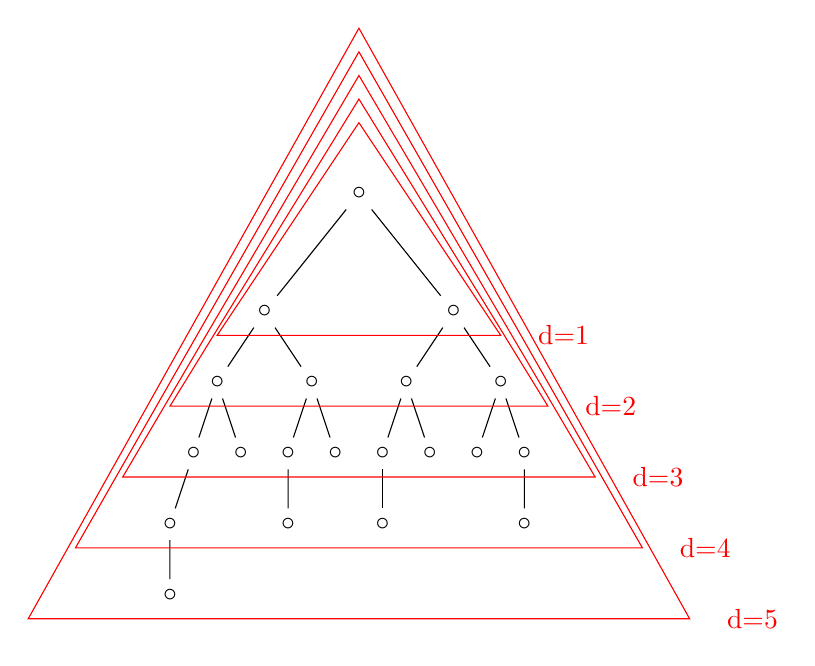
\begin{tikzpicture}[scale=.6]
\draw  (0,4) node (v1) {$\circ$};
\draw  (-2,1.5) node (v2) {$\circ$};
\draw  (2,1.5) node (v7) {$\circ$};
\draw  (-3,0) node (v3) {$\circ$};
\draw  (-1,0) node (v4) {$\circ$};
\draw  (1,0) node (v8) {$\circ$};
\draw  (3,0) node (v11) {$\circ$};
\draw  (-3.5,-1.5) node (v16) {$\circ$};
\draw  (-2.5,-1.5) node (v22) {$\circ$};
\draw  (-1.5,-1.5) node (v5) {$\circ$};
\draw  (-0.5,-1.5) node (v6) {$\circ$};
\draw  (3.5,-1.5) node (v13) {$\circ$};
\draw  (2.5,-1.5) node (v12) {$\circ$};
\draw  (1.5,-1.5) node (v10) {$\circ$};
\draw  (0.5,-1.5) node (v9) {$\circ$};
\draw (v1) -- (v2) -- (v3) -- (v16) (v2) -- (v4);
\draw (v4) -- (v5) (v3) -- (v22) (v4) -- (v6) (v1) -- (v7) -- (v8) -- (v9) (v8) -- (v10) (v7) -- (v11) -- (v12) (v11) -- (v13);
\draw  (-4,-3) node (v17) {$\circ$};
\draw  (-4,-4.5) node (v18) {$\circ$};
\draw  (-1.5,-3) node (v19) {$\circ$};
\draw  (0.5,-3) node (v20) {$\circ$};
\draw  (3.5,-3) node (v21) {$\circ$};
\draw [red](-3,1) -- (3,1)node[right = 1em]{d=1} -- (0,5.5) -- cycle;
\draw [red](-4,-0.5) -- (4,-0.5)node[right = 1em]{d=2} -- (0,6) -- cycle;
\draw (v16) -- (v17) -- (v18);
\draw (v5) -- (v19);
\draw (v9) -- (v20);
\draw (v13) -- (v21);
\draw [red] (-5,-2) -- (5,-2)node[right = 1em]{d=3} --(0,6.5) -- cycle;
\draw [red](-6,-3.5) -- (6,-3.5)node[right = 1em]{d=4} -- (0,7) -- cycle;
\draw [red](-7,-5) -- (7,-5)node[right = 1em]{d=5} -- (0,7.5) -- cycle;
\end{tikzpicture}
\end{center}
Die iterative Tiefensuche besitzt damit alle Vorteile.\\
Zur Rechenzeit: Diese ist länger als bei der Breitensuche, da alle vorherigen Kanten nochmal besucht werden.\\
In einem Suchbaum mit Verzweigungsfaktor $>1$ sind fast alle Knoten Blätter. Daher fällt auch die meiste Rechenzeit für das Durchsuchen der Blätter an. Durch eine genaue Rechnung lässt sich zeigen, dass die Laufzeit der iterativen Tiefensuche nur um einen kleinen Faktor höher ist als die der Tiefensuche.

\begin{lstlisting}[language=Prolog]
% Node: aktueller Knoten
% Goal: Zielknoten
% Path: Liste der Knoten auf dem Pfad bis Node
% ReturnPath: Rückgabe, wenn ein Pfad zum Ziel gefunden wurde
dlDfs(Node, Goal, Path, DepthLimit, ReturnPath) :-
	Node = Goal, reverse(Path, ReturnPath);
	DepthLimit > 0,
	adj(Node,NewNeighbor), not(member(NewNeighbor,Path)),
	dlDfs(NewNeighbor, Goal, [NewNeighbor|Path], DepthLimit-1, ReturnPath).

idDfsLoop(Start, Goal, D, ReturnPath) :-
	dlDfs(Start, Goal, [Start], D, ReturnPath);
	% Wenn die Tiefensuche mit Schranke D nicht erfolgreich war, wird mit Schranke D+1 weitergesucht.
	idDfsLoop(Start, Goal, D+1, ReturnPath).

idDfs(Start, Goal, ReturnPath) :- idDfsLoop(Start, Goal, 1, ReturnPath).

\end{lstlisting}

\subsubsection{Anwendung: Planungsproblem}
Affe-Banane-Problem\\
Situation: Raum mit
\begin{itemize}
\item Affe an der Tür
\item Banane an der Decke in der Mitte des Raumes
\item Stuhl am Fenster
\end{itemize}
Ziel: Affe soll die Banane greifen.\\
Regeln: Affe kann laufen, den Stuhl verschieben, auf den Stuhl steigen, die Banane greifen, wenn er unter der Banane auf dem Stuhl steht.\\
Zugehöriger Graph, der das Suchproblem darstellt: Knoten sind Situationen, Kanten entsprechen den anwendbaren Regeln.
\begin{center}
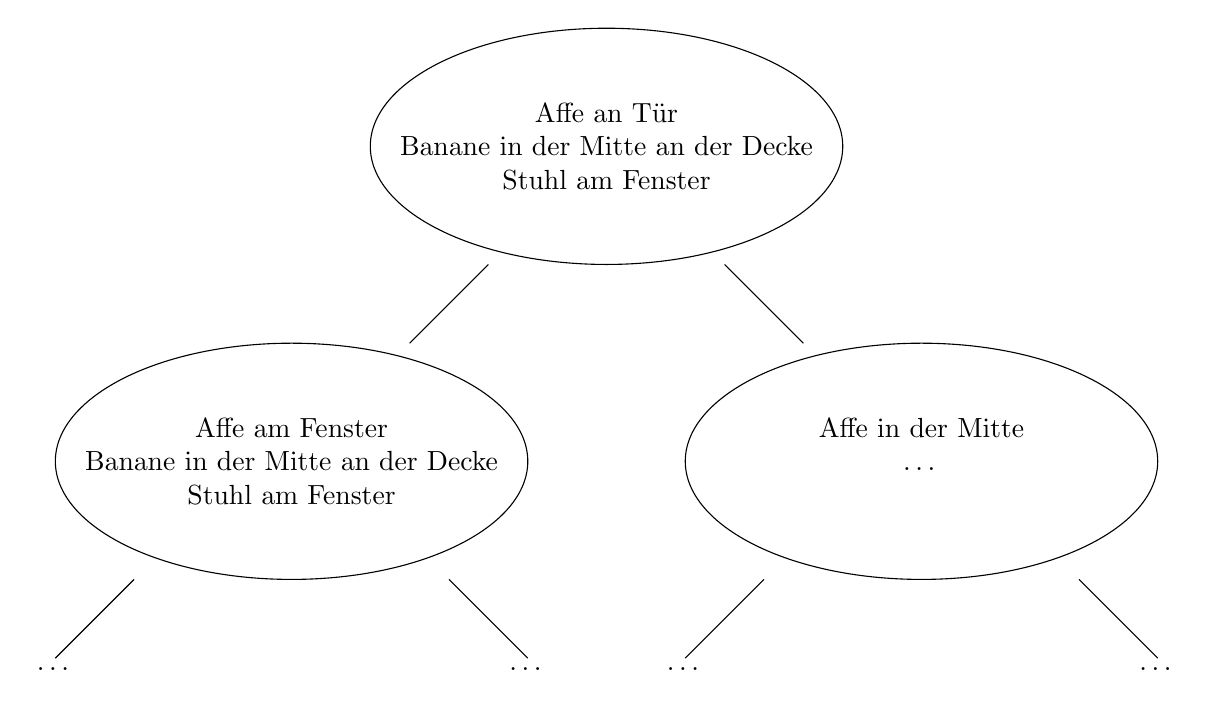
\begin{tikzpicture}[align= center]
\draw (0,0) node{Affe an Tür\\
Banane in der Mitte an der Decke\\
Stuhl am Fenster} ellipse (3 and 1.5);
\draw (-4,-4) node{Affe am Fenster\\
Banane in der Mitte an der Decke\\
Stuhl am Fenster} ellipse (3 and 1.5);
\draw (4,-4) node{Affe in der Mitte\\
…\\
~} ellipse (3 and 1.5);
\draw (-2.5,-2.5) -- (-1.5,-1.5);
\draw (2.5,-2.5) -- (1.5,-1.5);
\draw (-7,-6.5) node[below]{…} -- (-6,-5.5);
\draw (-1,-6.5) node[below]{…} -- (-2,-5.5);
\draw (1,-6.5) node[below]{…} -- (2,-5.5);
\draw (7,-6.5) node[below]{…} -- (6,-5.5);
\end{tikzpicture}
\end{center}

\begin{lstlisting}[language=Prolog]
:- [idDfs].	% entspricht include

ort(X) :- member(X, [tuer, mitte, fenster]).
% Bedeutung der Listen: [Affe, Banane, Stuhl, Affe auf Stuhl]
adj0([A1,B,S,f], [A2,B,S,f]) :- ort(A1), ort(A2).		% laufen
adj0([A1,B,A1,f], [A2,B,A2,f]) :- ort(A1), ort(A2).		% Stuhl schieben
adj0([A,B,A,f], [A,B,A,t]).		% auf Stuhl steigen
goal([A,A,_,t]).		% Banane greifen

adj(X,Y) :- adj0(X,Y); adj0(Y,X).

solution(Path) :- Start = [tuer, mitte, fenster, f], goal(Goal), idDfs(Start,Goal,Path).
\end{lstlisting}

\section{Informierte Suche (heuristische Suche)}
\lecdate{29.05.2017}
Ziel: Information über das Suchproblem nutzen, um gute Pfade zuerst zu verfolgen. Dabei wird eine Bewertungsfunktion für die Knoten verwendet.\\
Die heuristische Suche verwendet eine heuristische Bewertungsfunktion $f: V\to \RR_0^+$. Für den Zielknoten $v$ gilt $f(v)=0$. Die Knoten mit der niedrigsten Bewertung werden zuerst verfolgt.
\subsection{Gierige Suche} Verwendet in jedem Schritt den Knoten, der dem Ziel am nächsten liegt.

\cparagraph{Beispiel} Suche nach kürzestem Weg zu einem Ort $f(v)=\text{Luftlinienentfernung zum Ziel}$
\begin{center}
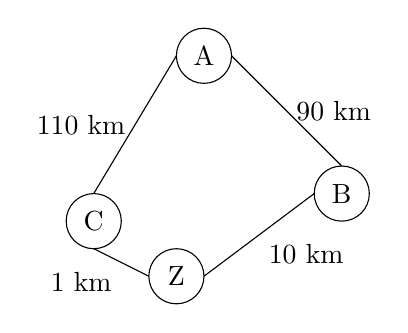
\begin{tikzpicture}[scale=.7]
\draw  (-2.5,2.5) node{A} ellipse (0.5 and 0.5);
\draw  (-4.5,-0.5) node{C} ellipse (0.5 and 0.5);
\draw  (0,0) node{B} ellipse (0.5 and 0.5);
\draw  (-3,-1.5) node{Z} ellipse (0.5 and 0.5);
\draw (-3,2.5) -- node[left]{110 km} (-4.5,0);
\draw (-4.5,-1) -- node[below left]{1 km} (-3.5,-1.5);
\draw (-2,2.5) -- node[right]{90 km} (0,0.5);
\draw (-2.5,-1.5) -- node[below right]{10 km} (-0.5,0);
\end{tikzpicture}
\end{center}
Die gierige Suche verfolgt den Weg A--C--Z (111 km). Dabei ist A--B--Z (100 km) kürzer.

\subsection{A*-Suche}
Die gierige Suche berücksichtigt nicht die Kosten, die bis zum Knoten $v$ bereits entstanden sind. Wir führen daher eine Funktion $g$ ein, die die Kosten vom Startknoten bis $v$ angibt (also der bereits zurückgelegte Weg) und eine Funktion $h$, die die (verbleibenden) Kosten bis zum Ziel schätzt.\\
Daher definieren wir die heuristische Bewertungsfunktion $f$ durch:
$$f(v)=g(v)+h(v)$$
Der A*-Algorithmus verwendet eine Bewertungsfunktion $f$, die die Summe der Kosten bis $v$ und die geschätzten Kosten bis zum Ziel sind. Dabei muss $h$ zulässig sein.
\cparagraph{Definition} Eine heuristische Kostenschätzfunktion $h$ heißt \emph{zulässig}, wenn $h$ die Kosten bis zum Ziel nie überschätzt.
\cparagraph{Beispiel}
\begin{itemize}
\item Die Luftlinienentfernung bis zum Ziel ist eine zulässige Kostenschätzfunktion.
\item $0$ (aber nicht nützlich, $\to$ gierige Suche).
\end{itemize}
\bigskip

\subsubsection{Implementierung durch Liste (ineffizient)}
Für jeden aktuellen Konten $u$ werden die noch unbesuchten Nachbarn $v$ bestimmt und diese entsprechend ihrer $f$-Werte sortiert in eine Liste der nach zu besuchenden Knoten eingefügt. Wenn die Liste dabei in jedem Schritt neu sortiert wird, entsteht jeweils ein Aufwand von $O(n \log n)$.
\subsubsection{Implementierung durch Min-Heap}
Eine effiziente Implementierung verwendet einen \emph{Min-Heap}.\\
Ein Min-Heap ist ein Binärbaum, in dem jeder Knoten, der kein Blatt ist, einen kleineren oder maximal gleichen Wert besitzt als alle Nachfolger.
\cparagraph{Beispiel}
\begin{center}
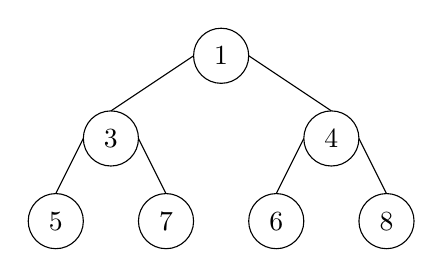
\begin{tikzpicture}[scale=.7]
\draw  (-1,3.5) node{1} ellipse (0.5 and 0.5);
\draw  (-3,2) node{3} ellipse (0.5 and 0.5);
\draw  (1,2) node{4} ellipse (0.5 and 0.5);
\draw  (-4,0.5) node{5} ellipse (0.5 and 0.5);
\draw  (-2,0.5) node{7} ellipse (0.5 and 0.5);
\draw  (0,0.5) node{6} ellipse (0.5 and 0.5);
\draw  (2,0.5) node{8} ellipse (0.5 and 0.5);
\draw (-1.5,3.5) -- (-3,2.5);
\draw (-3.5,2) -- (-4,1);
\draw (-2.5,2) -- (-2,1);
\draw (-0.5,3.5) -- (1,2.5);
\draw (0.5,2) -- (0,1);
\draw (1.5,2) -- (2,1);
\end{tikzpicture}
\end{center}
Alle wichtigen Heap-Operationen (\lstinline`readMin, add`) können in der Zeit $O(\log n)$ ausgeführt werden.\\
Eine effiziente A*-Suche verwendet einen Min-Heap, um die Knoten entsprechend ihrer $f$-werte zu verwalten. Dadurch fällt in jedem Schritt nur noch ein zusätzlicher Aufwand von $O(\log n)$ an.\bigskip\\
Die A*-Suche ist optimal, d.h., sie findet einen kürzesten Weg.

\subsubsection{Vor-/Nachteile}
\begin{itemize}
\item[$+$] Bei guter Heuristik wird das Ziel oft wesentlich schneller gefunden als mit einer uninformierten Suche.
\item[$-$] Hoher Speicherbedarf, weil im worst-Case alle Knoten gespeichert werden müssen.
\item[$-$] (wie bei Breitensuche:) es ist nicht einfach möglich den gefundenen Pfad zurückzugeben. 
\end{itemize}

%%% TODO Quellcode einfügen















